
%%%%%%%%%%%%%%%%%%%%%%%%%%%%%%%%%%%%%%%%%%%%%%%%%%%%%%%%%%
\chapter{Related Work}
\label{chapter_related_work}
%%%%%%%%%%%%%%%%%%%%%%%%%%%%%%%%%%%%%%%%%%%%%%%%%%%%%%%%%%

\mynote{
\begin{packeditems}
\item More than a literature review
\item Organize related work - impose structure
\item Be clear as to how previous work being described relates to your own. This is not just a list of the related work, you must describe how it is related. How is similar? How is it different?
\item The reader should not be left wondering why you've described something!!
\item Critique the existing work - Where is it strong where is it weak? What are the unreasonable/undesirable assumptions?
\item Identify opportunities for more research (i.e., your thesis) Are there unaddressed, or more important related topics?
\item After reading this chapter, one should understand the motivation for and importance of your thesis
\item You should clearly and precisely define all of the key concepts dealt with in the rest of the thesis, and teach the reader what s/he needs to know to understand the rest of the thesis.
\end{packeditems}
}

\mynote
{
	because it's deformation-driven thesis, 
	you need to explain deformation-driven packing vs rigid packing vs data driven packing
}

\begin{figure}[t]
\centering
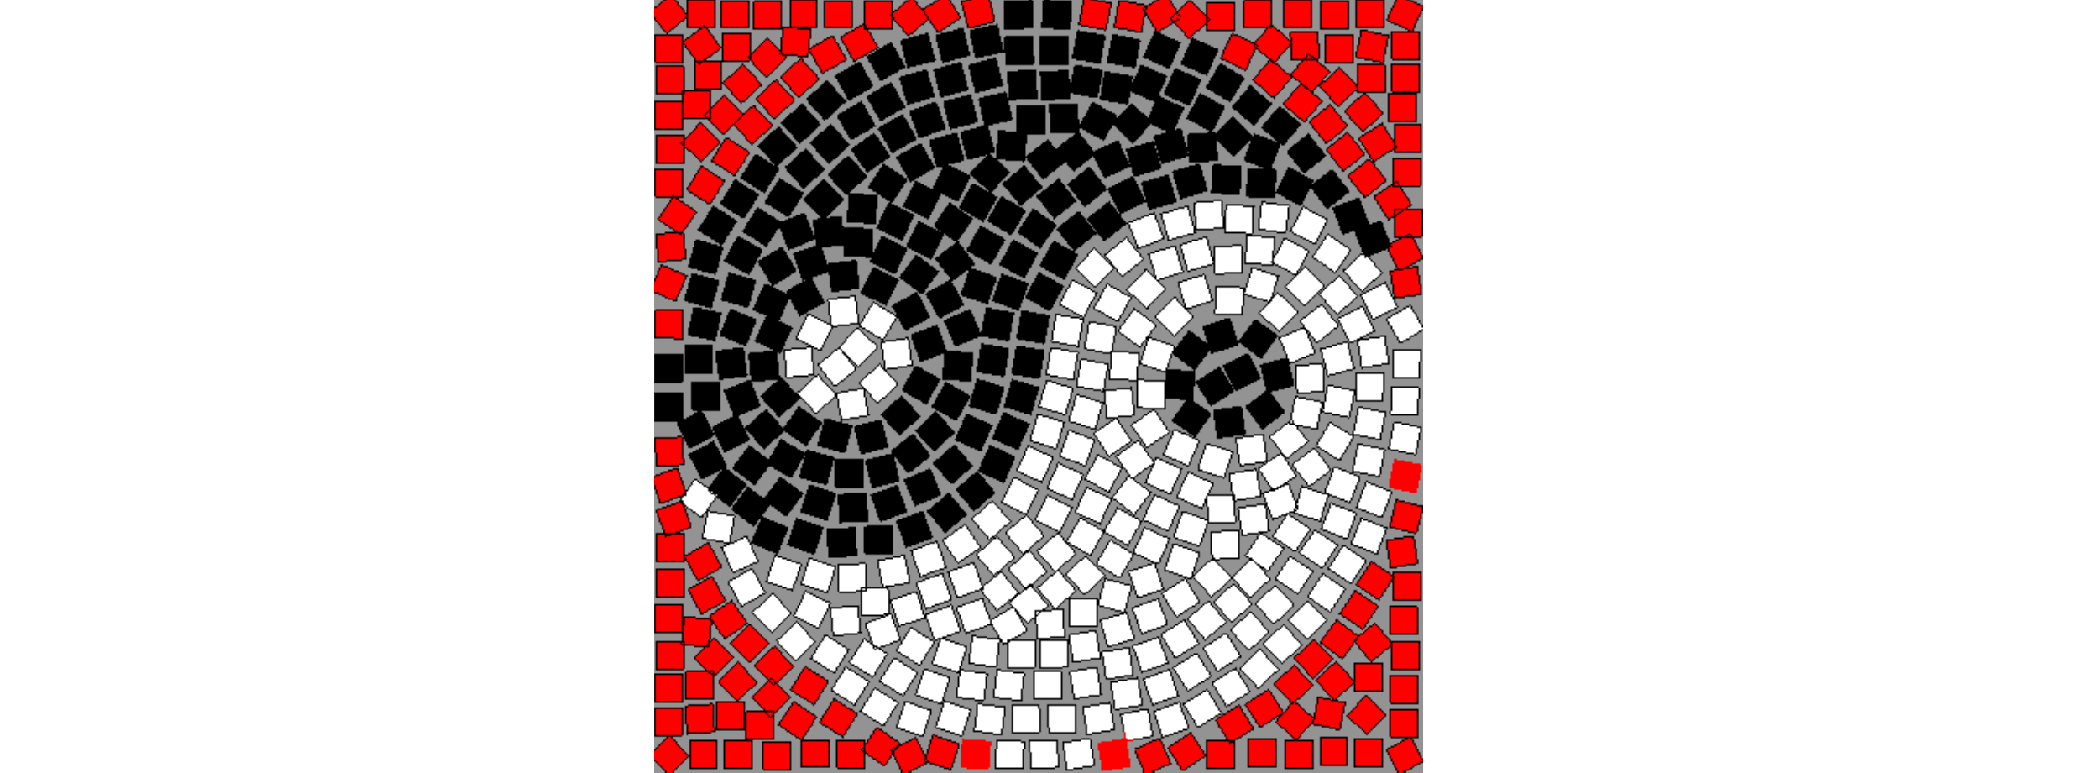
\includegraphics[width=1.0\textwidth]{figures/related/hausner.pdf} 
\caption[Decorative mosaics using Lloyd's method]
{\label{fig_related_hausner} 
Hausner. }
\end{figure}


\begin{figure}[t]
\centering
\includegraphics[width=1.0\textwidth]{figures/related/jim_pad.pdf} 
\caption[Examples of packings generated by JIM and PAD]
{\label{fig_related_jim_pad} 
JIM and PAD. }
\end{figure}

\begin{figure}[t]
\centering
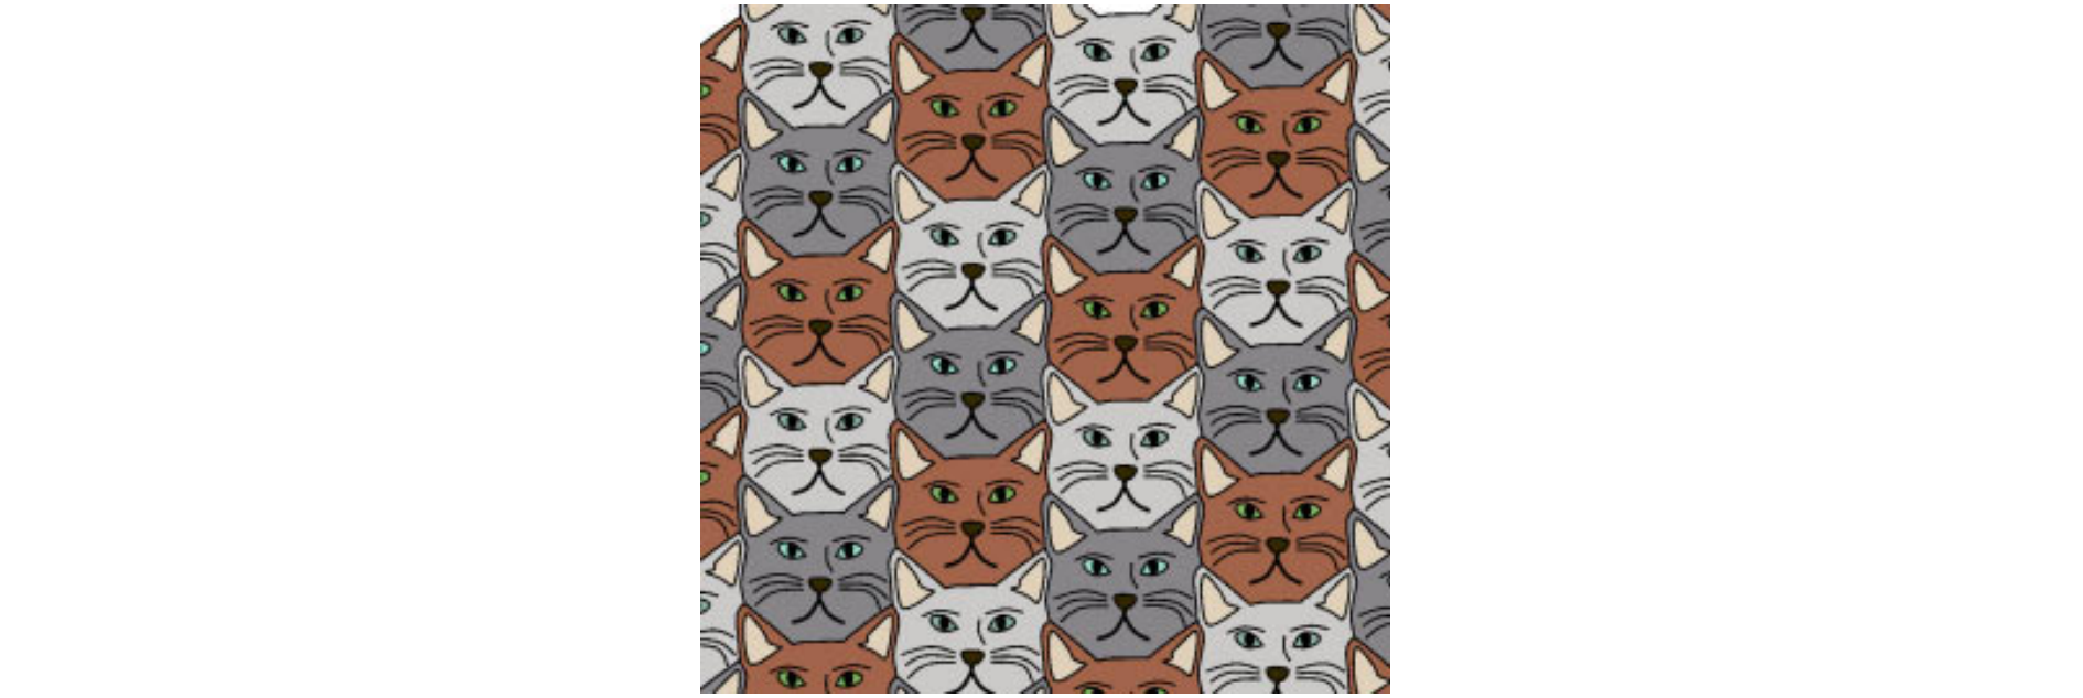
\includegraphics[width=1.0\textwidth]{figures/related/escherization.pdf} 
\caption[An example of a tiling]
{\label{fig_related_escherization} 
A tiling of cats. }
\end{figure}

\begin{figure}[t]
\centering

\includegraphics[width=1.0\textwidth]{figures/related/zehnder.pdf} 
\caption[An example of decorative ornaments filling a surface]
{\label{fig_related_zehnder} 
An example of decorative ornaments filling a surface.}
\end{figure}

\begin{figure}[t!]
\centering

\includegraphics[width=1.0\textwidth]{figures/related/calligraphy.pdf} 
\caption[A calligraphy packing of an ``elephant'']
{\label{fig_calligraphy} 
A calligraphy packing of an ``elephant'.}
\end{figure}


\textbf{Rigid packings using Lloyd's method:}
Lloyd's method is a technique to create an even distribution of \textit{sites}.
Given an initial distribution of $N$ sites, we first compute a Voronoi diagram to partition the plane into $N$ regions.
All points inside a Voronoi cell are closest to its corresponding site.
Lloyd's method is an iterative process, we move every site point to the centroid of its Voronoi cell, then the Voronoi diagram is recomputed.
The process is repeated until the site points reach an even distribution.
Originally, Lloyd's method can only work if the sites are points.
Hausner~\cite{Hausner2001} modified the Lloyd's method to pack oriented square elements into a container 
region, simulating the appearance of traditional mosaics. 
This can be achieved by replacing Euclidean distance with Manhattan distance so that Voronoi cells resemble squares instead of hexagons.
Hiller et al.~\cite{Hiller2003} extended Hausner's idea to distribute polygonal
elements instead of points 


%%%%%%%%%%%%%%%%%%%%%%%%%%%%%%%%%%%%%%%%%%%%%%%%%%%%%%%%%%

\mynote{explain Llyod's method, voronoi diagram and manhattan voronoi diagram}
\textbf{Rigid packings:}
The ever-popular Lloyd's method~\cite{McCool1992}
is an iterative
process for creating a perceptually even distribution of points, and has been
used in various forms in procedural packing methods.
Hausner~\cite{Hausner2001} 
used a variant of Lloyd's method to pack oriented rectangles into a container 
region, simulating the appearance of traditional mosaics.  
Hiller et al.~\cite{Hiller2003} extended Lloyd's method to distribute polygonal
elements instead of points, reducing the overlaps in Hausner's approach.
Dalal et al.~\cite{Dalal2006} used an FFT-based image correlation to reposition
elements iteratively, which could be seen as making more effective use of negative
space, and permitting non-convex elements to interlock more than they did in
earlier methods.
\mynote{add smith, and how they reorient tiles?}


%%%%%%%%%%%%%%%%%%%%%%%%%%%%%%%%%%%%%%%%%%%%%%%%%%%%%%%%%%
\textbf{Data-driven packing:}
JIM and PAD methods require an element database to make their algorithms works.
JIM uses geometric hashing to find a matching element, 
while PAD uses a partial shape matching algorithm.
Huang et al.~\cite{Huang2011} produced Arcimboldo-like collages
by searching a matching element from a 2D cutout image database collected from the internet.  
The more elements in the database will increase their chance to \textbf{find a compatible element boundary}.
However, bigger database means increased computational time.
Collecting a large number of elements is also not always feasible,
for example, if an artist wants to create a packing of a hand-drawn cats,
they may not want to draw 1000 cats which is tedious and repetitive.
\mynote{we use small sized database, sometimes only one or two elements, create compatible element boundary, 
generate variety through deformation}
%Huang et al.~\cite{Huang2011} produced Arcimboldo-like
%collages in 2D by layering objects cut out from images on top of a
%segmented container.  These methods benefit from overlaps, which
%join elements into a single large object.

%%%%%%%%%%%%%%%%%%%%%%%%%%%%%%%%%%%%%%%%%%%%%%%%%%%%%%%%%%
\textbf{Non-rigid packings:}
JIM~\cite{Kim2002} deformed elements
only in their post-processing step, which is to improve their results due to limitations in their algorithm.
Peng et al.~\cite{Peng2014} computed layouts by packing and deforming
simple polygons and polyominoes. Their method cannot handle more
complicated shapes, making it unsuitable for our style of packings.
Xu and Kaplan~\cite{Xu2007} and Zou et al.~\cite{Zou2016}
constructed \textit{calligrams} by filling a container with a small
number of deformed letters composing one or two words.  Because the
order of the letterforms was defined by the text, their solutions
usually required significant distortion of the individual letters.
Their goal was to balance between filling the container and preserving
readability.
Zehnder et al.~\cite{Zehnder2016} proposed an method to
cover 3D surfaces with deformed ornamental elastic curves.



%%%%%%%%%%%%%%%%%%%%%%%%%%%%%%%%%%%%%%%%%%%%%%%%%%%%%%%%%%
\mynote{dihedral escherization}
\textbf{Tilings:}
Kaplan and Salesin~\cite{Kaplan2000} deformed a single user-supplied 
input shape into one that could tile the plane.

%%%%%%%%%%%%%%%%%%%%%%%%%%%%%%%%%%%%%%%%%%%%%%%%%%%%%%%%%%
\textbf{3D packings:}
Gal et al.~\cite{Gal2007B} presented a method for constructing 3D
collages reminiscent of portrait paintings by Arcimboldo.  They
filled a 3D container with overlapping 3D elements using a greedy
approach and a partial shape matching algorithm.
Attene~\cite{Attene2015} decomposed a 3D model into parts that pack
tightly into a small build volume, allowing it to 
be 3D printed with less waste material and packed into a smaller box.
Ma et al.~\cite{Ma2018} developed a heuristic method
to create 3D packings that are overlap free.

%%%%%%%%%%%%%%%%%%%%%%%%%%%%%%%%%%%%%%%%%%%%%%%%%%%%%%%%%%
\textbf{Texture synthesis:}
Some past work has sought to adapt example-based texture synthesis methods
from raster images to vector graphics, producing distributions of rigidly transformed elements
that mimic the statistics of an exemplar.  Barla et al.~\cite{Barla2006} and
Ijiri et al.~\cite{Ijiri2008} use a growth model that copies small neighbourhoods
from the exemplar into a larger output texture.  AlMeraj et al.~\cite{AlMeraj2013}
stamp out copies of the exemplar and discard overlapping elements.
Hurtut et al.~\cite{Hurtut2009} develop a statistical sampling method based
on multitype point processes.  
These techniques are all concerned with replicating
the uneven element distribution in the exemplar, without regard for negative space.

%%%%%%%%%%%%%%%%%%%%%%%%%%%%%%%%%%%%%%%%%%%%%%%%%%%%%%%%%%
\textbf{Packings on manifolds:}
Related work in fabrication has sought to cover surfaces with
arrangements of deformed ornamental elements that satisfy manufacturing
constraints such as connectivity.  Chen et al.~\cite{Chen2016}
developed a method to synthesize filigree patterns out of simple
elements. 
In later work, Chen et al.~\cite{Chen2017}
generated modular surfaces by computing 
contact point networks of rigid elements.
\mynote{zehnder}




